%!TEX root = ../thesis.tex

\newcommand{\D}{\scr D}

\paragraph{notation}

We note that the interior of some cycle $\interior(C)$ are all vertices strictly in the interior of this cycle. We will sometimes also take $\interior(C)$ to refer to the induced subgraph of these vertices.

We let $\intplus(C)$ denote the the vertices of $C$ and $C$'s interior vertices. We will also sometimes let it refer to the subgraph of $G$ induced by these vertices.


\paragraph{coloring}
In this section we will use lots of figures to demonstra how to handle each type of $4$-cycle.


\section{Seperating 4 cycles}
Let $\D$ be a maximal separating $4$-cycle.

Note that the only problem is given by $4$-cycles that are entirely inside the cycle $\C$ maintained by the algorithm. If $\C$ is currently crossing $\D$ then the is not any longer a problem.

We can discern $7$ types of adjacency for $4$-cycles to a cycle if it's entirely inside some cycle.
\begin{enumerate}
  \renewcommand*{\labelenumi}{(\alph{enumi})}%
  \renewcommand*{\theenumi}{(\alph{enumi})}%

  \item $\D$ has $1$ edge on the cycle
  \label{t:1}
  \item $\D$ has 2 consecutive edges on the cycle
  \label{t:2cons}
  \item 2 non-consecutive edges on the cycle
  \label{t:2alt}
  \item 3 edges on the cycle
  \label{t:3}
  \item Just a vertex on the cycle
  \label{t:v1}
  \item Two consecutive vertices on the cycle
  \label{t:v2cons}
  \item Two non-consecutive vertices on the cycle
  \label{t:v2alt}
\end{enumerate}

We will show by case distinction that everything will be okay. Sometimes we will make a move (updating cycle and prefence) to remove a iregularity and sometimes this will not be necesarry.



We know that $\D \subseteq \intplus(\C)$. Either $\D \cap \C \neq \emptyset$ or
$\D \cap \C = \emptyset$. In the first case we will say that $\D$ is on the cycle.
In the second case we have that $\D \subseteq \intplus(\C_\F)$ since


\subsection{On the cycle}
  Note that type \ref{t:2alt}, \ref{t:3} and \ref{t:v2cons} can't occur on the cycle $\C$ maintained by the algorithm since they give a chord, offending Invariant \ref{i:noChords}.
  \paragraph{Type \ref{t:1}}
  This is a \emph{short chord}. Note that we allow a choiche of edge flip to be made after

  \paragraph{Type \ref{t:2cons}}
  We can do a simple move evading the problem.
  %But maybe a normal algo run will also work. However for the normal algo we assume no 4-cycles, so we should do this separately.

  We make the move depicited in Figure \ref{fig:4c:cycle_b}
  \begin{figure}[h]
    \centering
    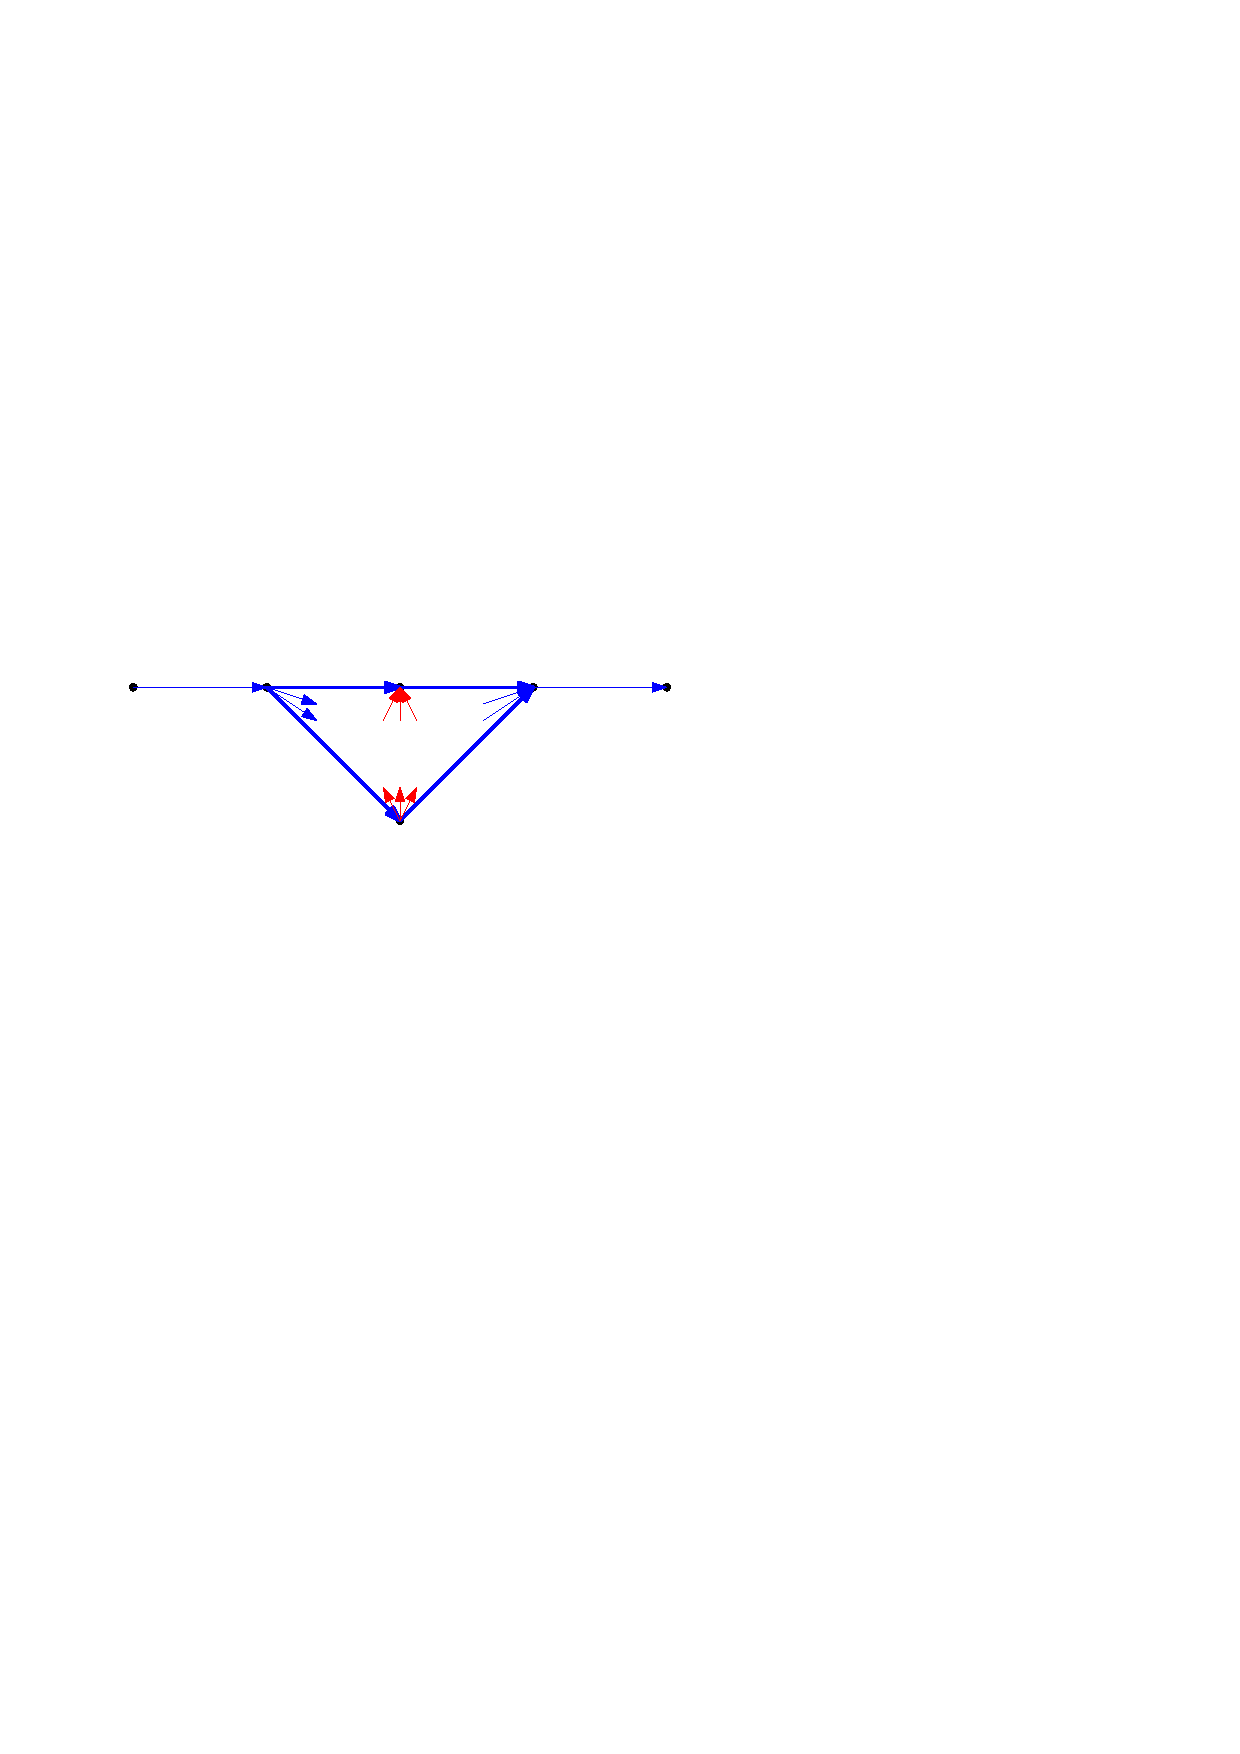
\includegraphics[scale=1]{4cycles/img/cycle_b}
    \caption{Removing a Type \ref{t:2cons} seperating $4$-cycle}
    \label{fig:4c:cycle_b}
  \end{figure}

  This moves the the cycle $\C$ past the problematic $4$-cycle $\D$. Note that we don't allow any freedom in the interior edges in this case.

  \paragraph{Type \ref{t:v1}}
  This type of separating $4$-cycle does not induce a irregularity in the fence. Hence no operation is necessary. 
  This is no problem, we can just ''corner-slice" it. This seperating $4$ cycle is no problem since it produces no irregularity on the (pre)fence $\W$.

  \paragraph{Type \ref{t:v2alt}}
  This is just a combination of a ordinary non-simple point and a Type \ref{t:2cons} case. If we first recurse on the inner non-simple point we can then solve the rest like the Type \ref{t:2cons} case.

\subsection{On the fence}
  \paragraph{Type \ref{t:1}}
  This is a \emph{short chord}


  \paragraph{Type \ref{t:2cons}}

  \paragraph{Type \ref{t:2alt}}

  \begin{figure}[h]
    \centering
    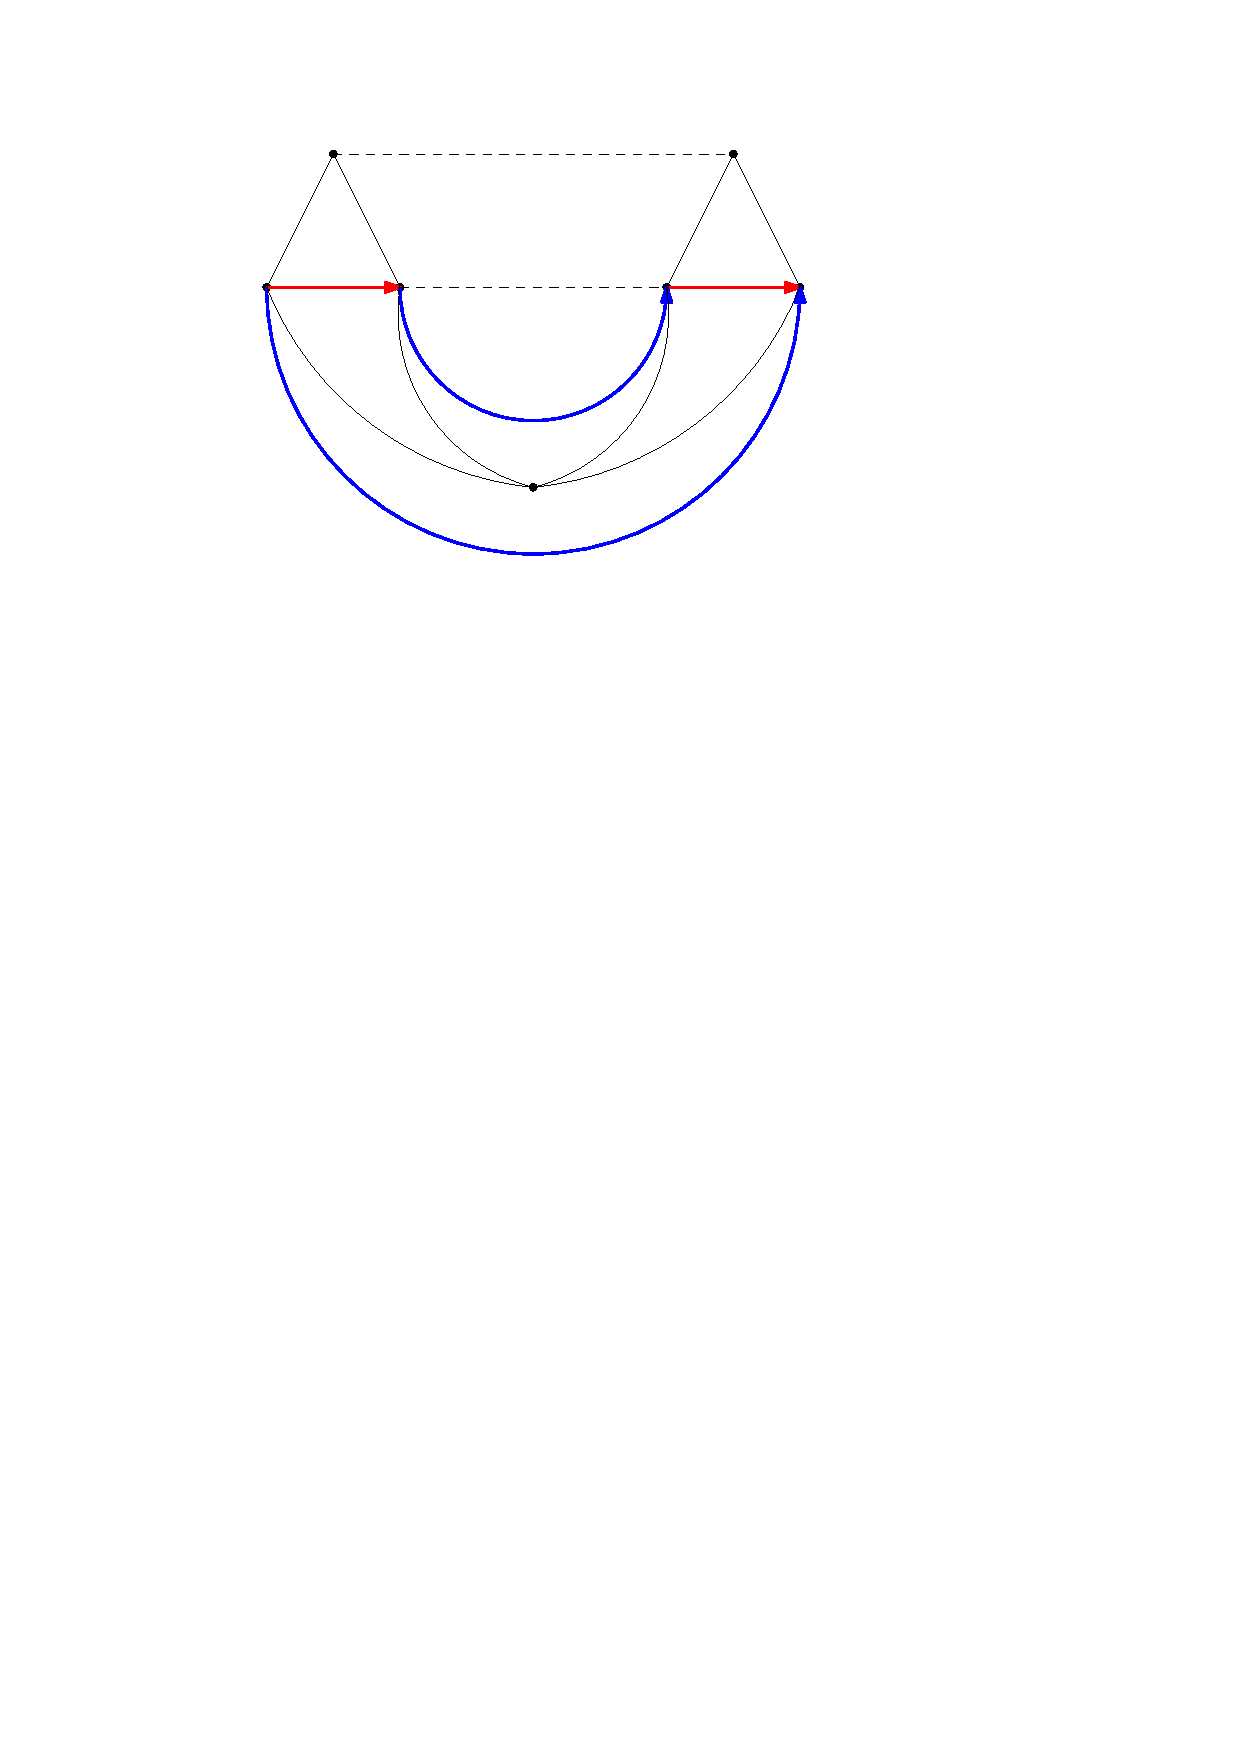
\includegraphics[scale=1]{4cycles/img/fence_c}
    \caption{}
    \label{fig:4c:fence_c}
  \end{figure}

  \paragraph{Type \ref{t:3}}

  \begin{figure}[h]
    \centering
    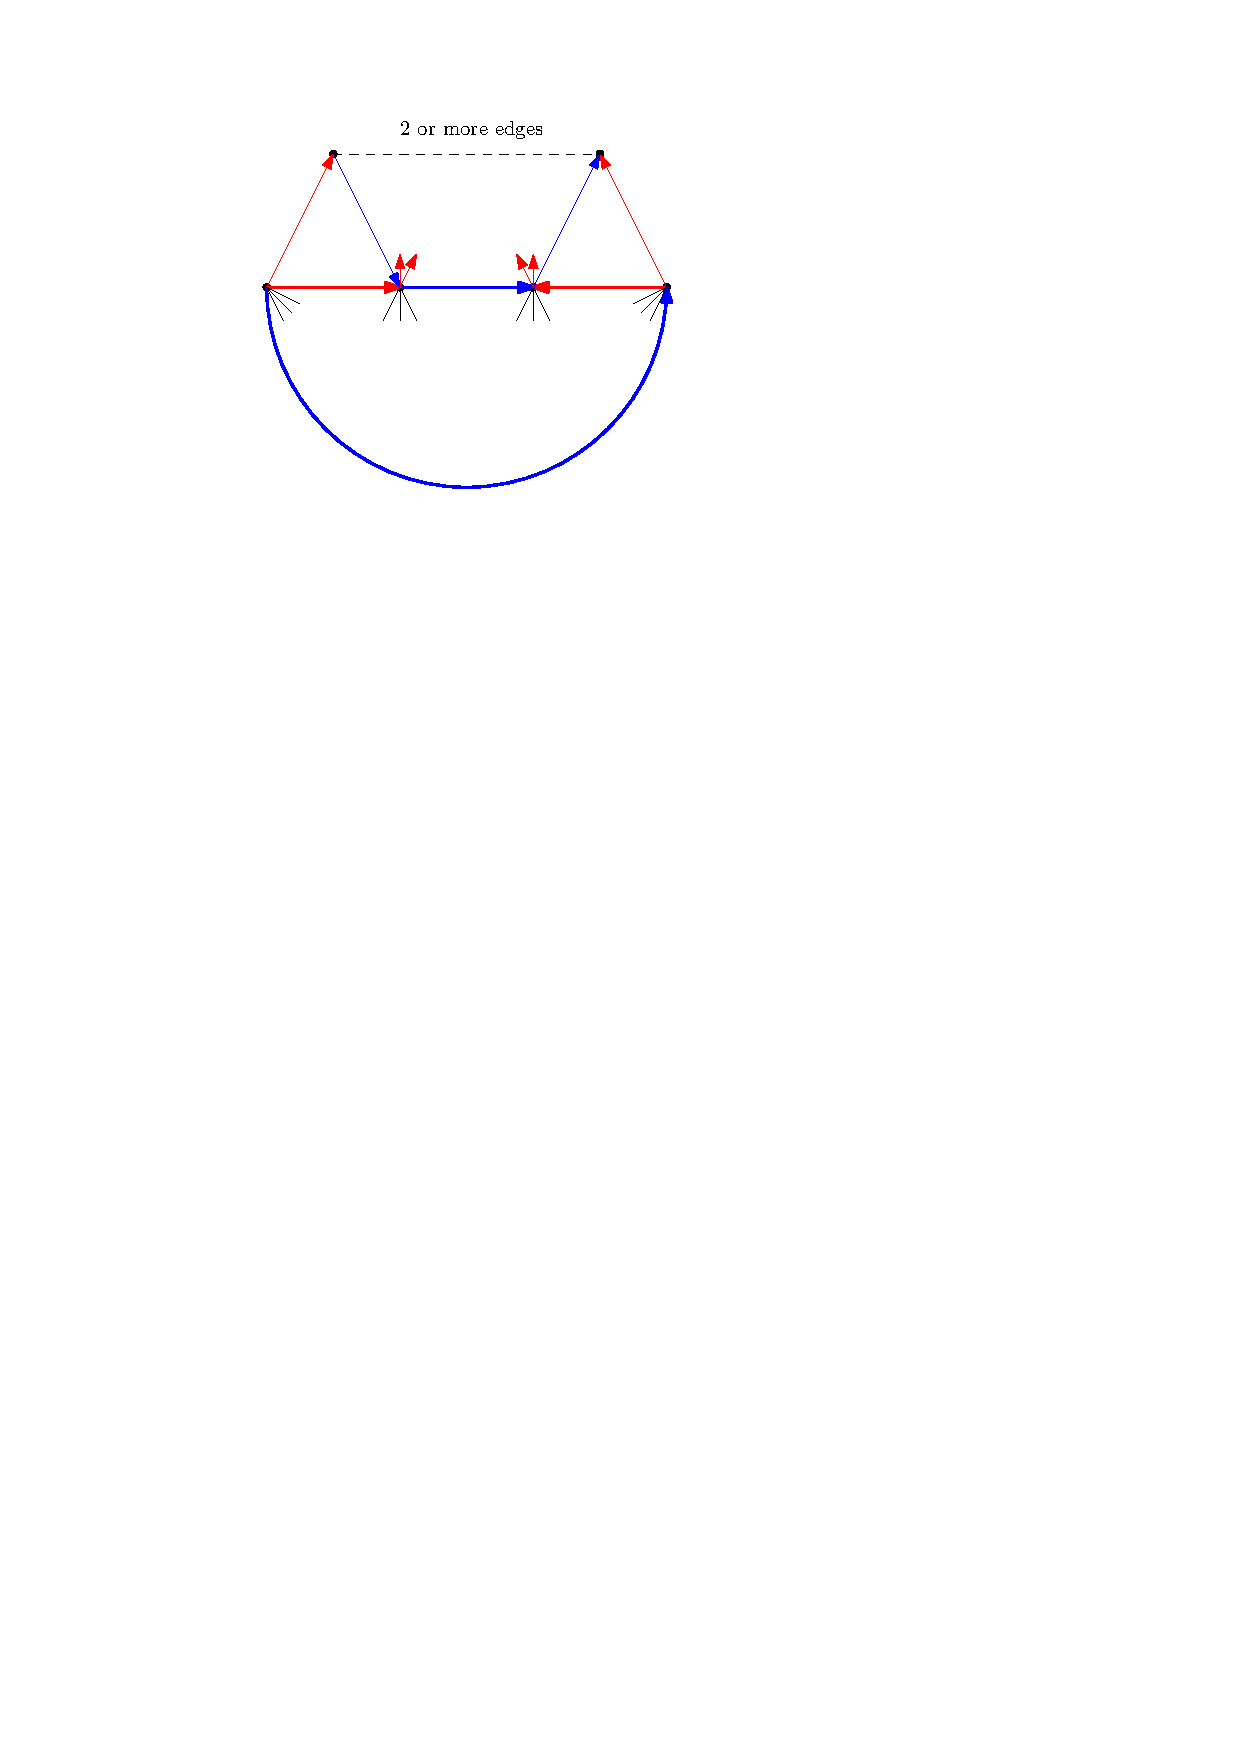
\includegraphics[scale=1]{4cycles/img/fence_d}
    \caption{}
    \label{fig:4c:fence_d}
  \end{figure}


  \paragraph{Type \ref{t:v1}}

  \paragraph{Type \ref{t:v2alt}}

  \paragraph{Type \ref{t:v2cons}}
    This is the inside of a chord

\subsection{Not on the cycle or on the fence}
  Then $\D$ is no problem.

\subsection{$4$-cycles with a complicated interior}
  We can just recurse

\subsection{Adjecent 4-cycles}
